\documentclass[12pt,oneside,bibtotoc,liststotoc]{scrbook}
\usepackage[utf8]{inputenc}
\usepackage{graphicx}
\usepackage[ngerman,german]{babel}
\usepackage{a4wide}
\usepackage{parskip}
\usepackage[bookmarks]{hyperref}
\usepackage{fancyhdr}
\usepackage[right]{eurosym}
\usepackage{amsmath}
\usepackage[toc,page]{appendix}
\usepackage{float}
\usepackage{tabularx}
\usepackage{booktabs}
\usepackage{pifont}

\newcommand{\cmark}{\ding{51}}

\usepackage[numbers]{natbib}
\DeclareUnicodeCharacter{2192}{ to}

\usepackage{lstautogobble}

\usepackage{array}
\usepackage{longtable}
\usepackage{listings}
\usepackage{color}
\usepackage[usenames,dvipsnames]{xcolor}
\colorlet{punct}{red!60!black}
\definecolor{background}{HTML}{EEEEEE}
\definecolor{delim}{RGB}{20,105,176}
\colorlet{numb}{magenta!60!black}
\lstdefinelanguage{json}{
    basicstyle=\footnotesize\ttfamily,
    numbers=left,
    tabsize=2,
    lineskip={-1.0pt},
    numberstyle=\scriptsize,
    stepnumber=1,
    numbersep=8pt,
    showstringspaces=false,
    breaklines=true,
    frame=lines,
    backgroundcolor=\color{background},
    literate=
      *{:}{{{\color{punct}{:}}}}{1}
      {,}{{{\color{punct}{,}}}}{1}
      {\{}{{{\color{delim}{\{}}}}{1}
      {\}}{{{\color{delim}{\}}}}}{1}
      {[}{{{\color{delim}{[}}}}{1}
      {]}{{{\color{delim}{]}}}}{1},
}
\lstdefinelanguage{rdf}{
    basicstyle={\footnotesize\ttfamily},
    lineskip={-1.0pt},
    numbers=left,
    numberstyle=\scriptsize,
    stepnumber=1,
    numbersep=8pt,
    showstringspaces=false,
    breaklines=true,
    frame=lines,
    tabsize=2,
    backgroundcolor=\color{background},
    keywordstyle={\bfseries\color{Blue}},
    commentstyle={\color{Red}\textit},
    stringstyle=\color{Magenta},
    morekeywords={ql,rml,rr,schema},
    moredelim=*[s][\ttfamily]{:}{:} %Newly added line
}
\lstdefinelanguage{xml}{
    basicstyle={\footnotesize\ttfamily},
    lineskip={-1.0pt},
    numbers=left,
    tabsize=2,
    numberstyle=\scriptsize,
    stepnumber=1,
    numbersep=8pt,
    showstringspaces=false,
    breaklines=true,
    frame=lines,
    backgroundcolor=\color{background},
    keywordstyle={\bfseries\color{Blue}},
    commentstyle={\color{Red}\textit},
    stringstyle=\color{Magenta},
    morekeywords={ServiceProvider,Document,Address,Service,Product,Occupancy,Price},
    moredelim=*[s][\ttfamily]{:}{:} %Newly added line
}
\newcommand\tab[1][1cm]{\hspace*{#1}}
\lstset{
	basicstyle=\ttfamily\small,
	showspaces=false,
	numbers=left,
	breaklines = true,
	showstringspaces=false
}

\pagestyle{headings}
\setlength{\textwidth}{15cm}
\setlength{\textheight}{22.5cm}
\setlength{\oddsidemargin}{1cm}
\setlength{\evensidemargin}{0cm}
\begin{document}

\thispagestyle{empty}
\begin{center}
\LARGE{Leopold-Franzens Universität Innsbruck\\
Fakultät für Mathematik, Informatik und Physik}\\[3ex]
\large{Institut für Informatik}
\end{center}
\medskip

\begin{center}
\begin{tabular}{c c}
\hspace{-1.5cm}
\includegraphics[height=3cm]{images/uibk_logo.jpg} &

\includegraphics[height=3cm]{images/EdgeAI_logo.png}
\end{tabular}
\vspace{1.5cm}


\textbf{\LARGE{Bachelorarbeit}}
\medskip\par
\textbf{\normalsize{zur Erreichung des akademischen Grades}} \\[3ex]
\textbf{\Large{Bachelor of Science}}
\vspace{2cm}

\textbf{\Large{Computer Vision for UAV Swarm Traffic Monitoring}}
\bigskip\par
von \par
\large{Dominik Schweigl}\\
(Matr.-Nr.: 12243381)
\end{center}
\vspace{1cm}

\begin{tabular}{ll}
  Submission Date:  & \today \\
  Univ.-Prof. Dr. Radu Prodan \\
\end{tabular}

\newpage


\vspace*{5cm}

\begin{center}
\LARGE{Eidesstattliche Erklärung}\\
\end{center}
\vspace{1cm}


\begin{quote}
\emph{Ich erkläre hiermit an Eides statt durch meine eigenhändige Unterschrift, dass ich die vorliegende Arbeit selbstständig verfasst und keine anderen als die angegebenen Quellen und Hilfsmittel verwendet habe. Alle Stellen, die wörtlich oder inhaltlich den angegebenen Quellen entnommen wurden, sind als solche kenntlich gemacht.
\\Ich erkläre mich mit der Archivierung der vorliegenden Bachelorarbeit einverstanden.
}
\end{quote}
\vspace{2.5cm}

\begin{flushleft}
\begin{tabular}{lll}
Ort und Datum: & & \rule{7cm}{0.4pt}\\[7ex]
Unterschrift: & & \rule{7cm}{0.4pt}
\end{tabular}
\end{flushleft}

\thispagestyle{empty}

\renewcommand{\baselinestretch}{1.00}\normalsize

\tableofcontents
\setcounter{page}{1}
\pagenumbering{Roman}
\listoffigures
\renewcommand{\baselinestretch}{1.5}\normalsize

\newpage
\setcounter{page}{1}
\pagenumbering{arabic}

\chapter*{Abstract}
\addcontentsline{toc}{chapter}{Abstract}

\begin{otherlanguage*}{english}
\end{otherlanguage*}





\chapter{Introduction}
Goes here...
\cite{karle2017semantify}

The remainder of this thesis is structured as follows. 
Chapter~\ref{chap:literature_review} provides a review of related 
literature on UAV-based traffic monitoring, sensor fusion, and aerial 
object detection. Chapter~\ref{chap:hardware} describes the hardware 
components employed in this work, including the UAV platform, the 
onboard processing unit, and the multi-sensor system, concluding with 
an overview of the overall system integration. 
Chapter~\ref{chap:sensor_fusion} discusses the theoretical foundations 
of sensor fusion, covering early, mid-level, and late fusion approaches 
as well as common challenges. Chapter~\ref{chap:object_detection} 
discusses object detection methods, including single-stage and 
two-stage detectors as well as tracking-by-detection paradigms. 
Chapter~\ref{chap:dataset} presents the dataset collected for this 
work. Chapter~\ref{chap:implementation} details the implementation 
of the detection system, encompassing RGB-thermal fusion, distance 
sensor integration, and edge optimization. 
Chapter~\ref{chap:evaluation} evaluates the proposed approach, 
followed by Chapter~\ref{chap:limitations}, which discusses its 
limitations. Finally, Chapter~\ref{chap:conclusion} summarizes the 
findings and outlines directions for future work.

\chapter{Literature Review}
\label{chap:literature_review}

% Literatur recherche

% Include graph of the number of papers per year over timespan

\chapter{Hardware}
\label{chap:hardware}

In this chapter, the hardware components relevant to the vehicle 
detection method developed in this thesis are described. The 
chapter begins with an 
introduction to the UAV platform, followed by a presentation of 
the onboard processing unit. Subsequently, the sensor system is 
examined through a comparison of relevant sensor modalities, 
providing justification for the selected approach. Finally, an 
overview of the overall system integration is provided.

\section{UAV Platform}

The aerial platform used in this work is the 
\textit{twinFOLD KAT}, a heavy-payload hexacopter developed by 
twins GmbH. According to the official product specification 
document \cite{twinsKATspec2021}, the system has a maximum takeoff 
weight of 12\,kg and supports a payload of up to 5.5\,kg 
including batteries and sensors. 

The UAV achieves a typical flight endurance of approximately 35 
minutes, with maximum flight times of up to 45 minutes under 
favorable conditions. The maximum horizontal flight speed is 
specified as 7\,m/s. Furthermore, the system is certified for 
operation in light rain or snowfall and supports missions up 
to 3000\,m above mean sea level, which allows for flights in
all tyrolian areas.
\cite{twinsKATspec2021}

\begin{figure}[H]
    \centering
    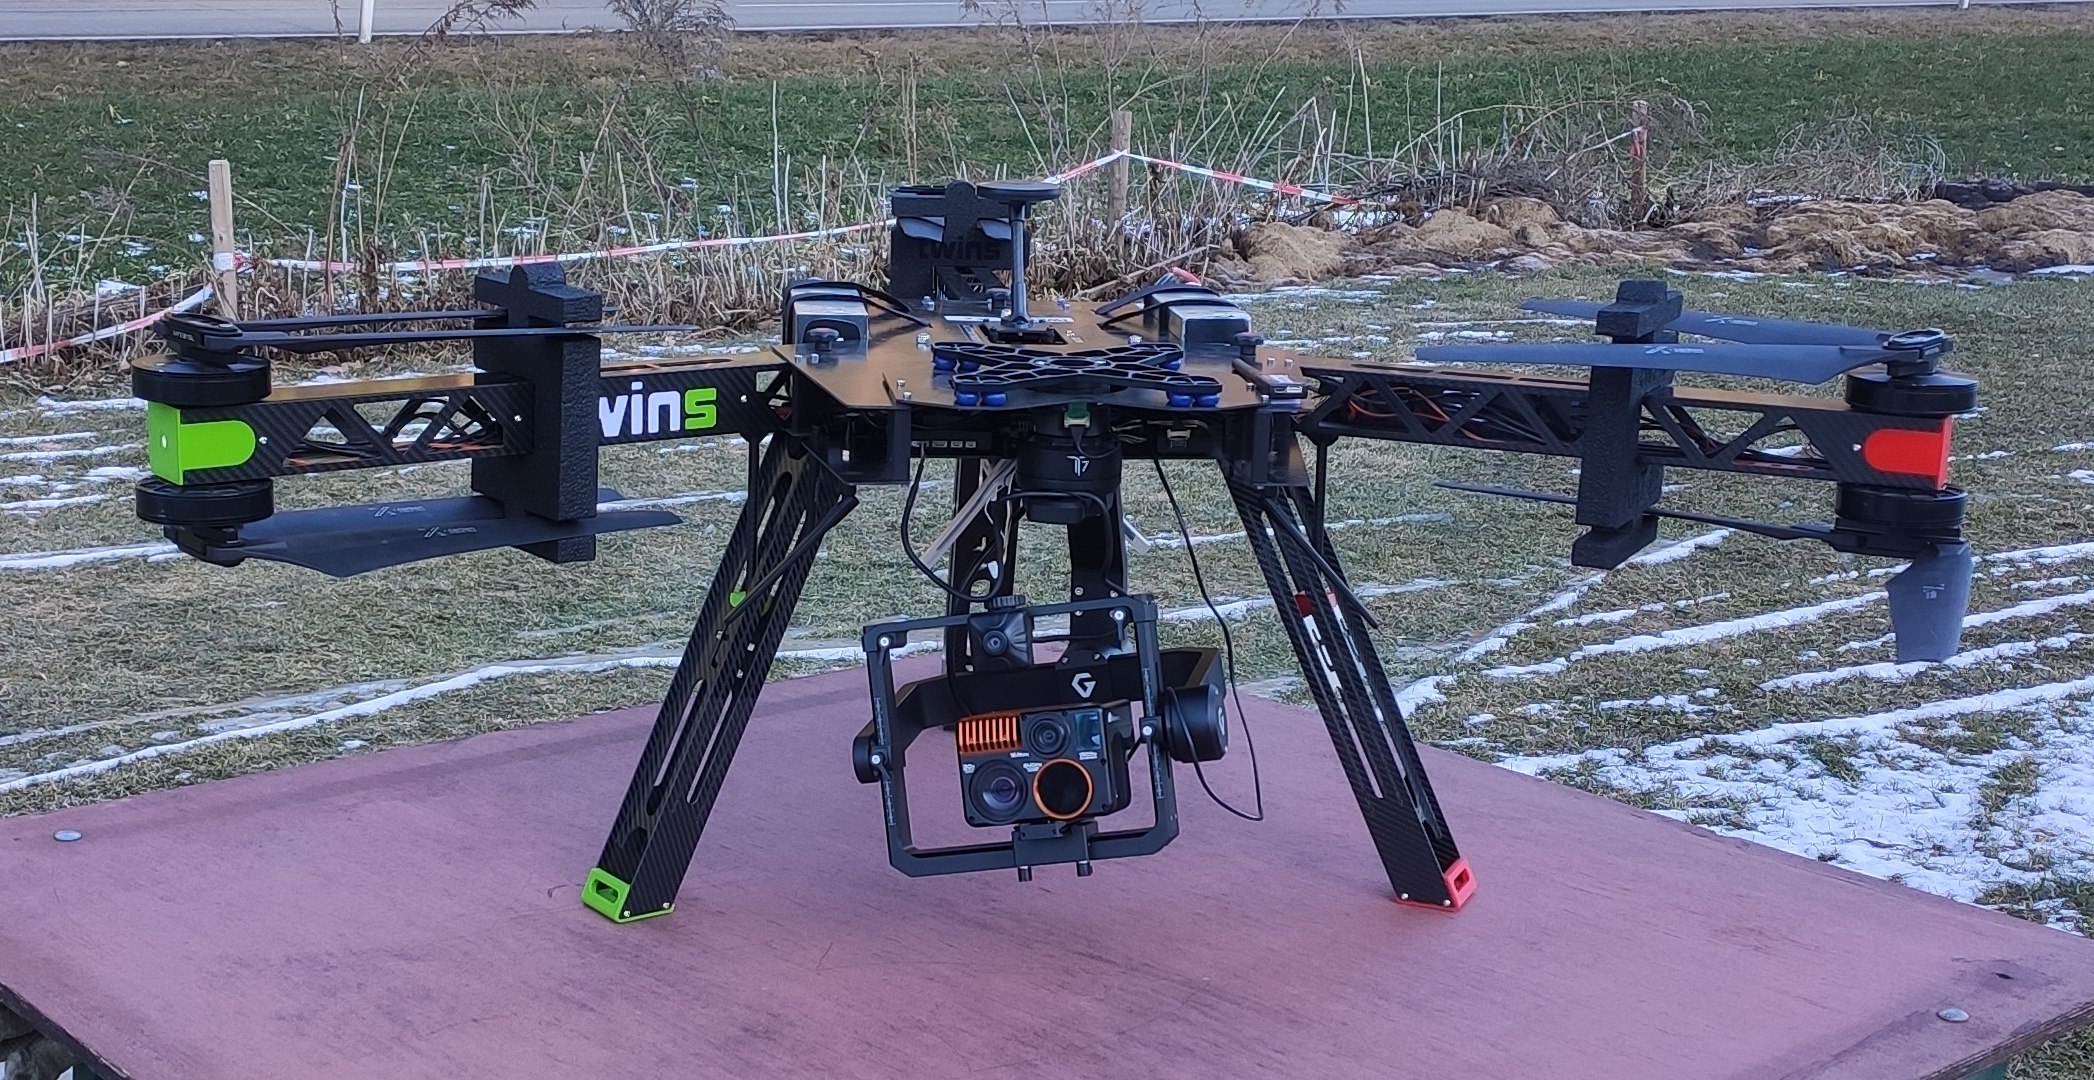
\includegraphics[width=0.65\textwidth]{images/twinFOLD_KAT.jpg}
    \caption{
        The twinFOLD KAT heavy-payload hexacopter including the 
        mounted sensor system on the first data collection mission.
    }
    \label{fig:twinFOLD_KAT}
\end{figure}


\section{Onboard Processing Unit}

Onboard data processing is performed using a 
\textit{Raspberry Pi 5} in combination with a 
\textit{Hailo AI accelerator}. This configuration enables 
real-time processing of multimodal sensor data directly on 
the UAV.

The Raspberry Pi 5 is equipped with a quad-core ARM 
Cortex-A76 CPU (up to 2.4\,GHz) and provides improved I/O 
performance compared to previous generations. It supports 
high-speed interfaces such as PCIe 2.0, which allows direct 
integration of external AI accelerators. Depending on the 
configuration, the system is available with up to 8\,GB of 
LPDDR4X RAM. Typical power consumption of the Raspberry Pi 5 
ranges between 5\,W and 12\,W, depending on workload and 
connected peripherals.

The Hailo accelerator (e.g., Hailo-8) is a dedicated deep 
learning inference processor designed for edge applications. 
It delivers up to 26 tera-operations per second (TOPS) while 
maintaining low power consumption (typically 2.5–3.5\,W under 
load). The accelerator is optimized for convolutional neural 
networks (CNNs) and supports common deep learning frameworks 
through a dedicated software development kit (SDK).

The combination of the Raspberry Pi 5 and the Hailo accelerator 
provides a compact and energy-efficient embedded computing 
platform capable of executing neural network-based vehicle 
detection algorithms in real time. This architecture enables 
onboard inference, reducing the need for high-bandwidth data 
transmission to a ground station and thereby increasing 
operational autonomy and system responsiveness.

\section{Sensor System}

The choice of the sensor system was primarily driven by the
selection of suitable data modalities for reliable vehicle
detection in aerial imagery and ease of integration. 
Several sensing modalities
were considered: RGB imaging, long-wave infrared (LWIR)
thermal imaging, LiDAR, and radar. Each modality offers
distinct advantages and limitations in terms of spatial
resolution, robustness to illumination changes, weather
tolerance, geometric information content, and computational
requirements. After modality evaluation, the selected
hardware \textit{Workswell WIRIS Enterprise} is described, 
including its specifications and the rationale for its selection.


\subsection{Modality Comparison}

Understanding the strengths and weaknesses of different sensing 
modalities is crucial for selecting the appropriate sensors for 
UAV-based vehicle detection. Each modality captures different 
aspects of the environment, and their performance can vary 
significantly under different environmental conditions. Here,
the most widely used modalities in object detection and 
autonomous perception are compared.

% TODO: Images for each modality, showing example detections and challenges

\paragraph{RGB Imaging}

Optical remote sensing is the oldest method of remote sensing.
It was started with the invention of photography. 
\cite{agrawal2019comparativeRemoteSensing}

RGB cameras provide high spatial resolution and rich texture
information, making them well suited for modern deep learning-
based object detection methods. They enable detailed scene
understanding and fine-grained classification. However, RGB
imaging strongly depends on ambient illumination and may
degrade significantly in low-light or night-time conditions.

The camera is a passive sensor that functions analogously
to the human eye, capturing reflected ambient light to form
a 2D image of the world. Its ubiquity, low cost, and high
resolution have made it an indispensable component of
transportation systems. While other sensors provide
geometric or motion data, the camera's unique strength lies
in its ability to deliver rich semantic and textural
information. It can distinguish colors, read text, and
recognize intricate patterns, allowing it to perform tasks that
are impossible for LiDAR or Radar, such as identifying
traffic light states, reading road signs, and detecting lane
markings [27]. The rapid advancement of deep learning and
convolutional neural networks has further unlocked the
camera's potential, enabling sophisticated scene
understanding and object classification from image data
alone.
\cite{soltanirad2025autonomousTransportationPerception}

In optical imaging, electromagnetic energy of the sun which is
reflected by the earth is received and measured. Its
electromagnetic spectrum range is from 0.4~$\mu$m to 1~mm. It is a
passive remote sensing technique. Hence it collects data only in
daytime. The incoming energy from earth is separated into
several spectral components that are sensed independently. The
light wave is directed from the grating through a prism that split
the energy into different wavelengths like UV, visible and near
infra-red. Multispectral image is a two dimensional (2D) array
of columns and rows of pixels. Each pixel contains digital
number that gives spectral reflection from the object of
particular band. Depending upon the number of bands it can be
multispectral or hyperspectral.
\cite{agrawal2019comparativeRemoteSensing}



On the other hand, data fusion techniques aim to synthesize the
information from different types of data (RGB, IR, LiDAR, radar) for
the same scene to increase their suitability for further image processing.
For instance, IR images can better reflect areas with high-temperature
contrast without being affected by dazzling light. In contrast, visible 
images can provide better details of the scene. Thus, fusing the two types
of images can combine the information and strengthen the performance
of the detection. Depending on the level of abstraction, the methods can
be applied to raw pixel data (low-level data fusion), extracted feature
data (medium-level data fusion), and/or combined classification data
from multiple sensors (decision-level data fusion).
\cite{bustos2023reviewObjectDetectionIR}

Detecting objects in RGB and IR images pose different types of challenges. 
Fig. 2 shows an example of key differences in object detection
on RGB and thermal images. For RGB images, lighting variations, color
confusion, and occlusions can make it difficult to accurately detect
objects. In contrast, IR images lack visual details, have a lower spatial
resolution, and are susceptible to environmental interference. Thus,
approaches that effectively combine and utilize the information from
different image modalities (i.e., fused RGB and thermal image) have the
potential to improve object detection. Understanding these challenges
and the methods that have been presented is crucial for developing
more effective object detection systems that leverage the strengths
of multiple imaging modalities while also considering their inherent
limitations.
\cite{bustos2023reviewObjectDetectionIR}

Cameras are cheap and small, but do not provide depth perception
capability and suffer from insufficient illumination or occlusions.
The camera's spatial resolution is naturally very high, in most cases higher
than millions of pixels per frame. Therefore, they can capture many semantic elements like color,
texture, and shape in a rich scene. However, the metric accuracy from cameras is inferred rather than
directly measured by stereovision or deep-learning-based depth estimation methods. Therefore, it is
affected easily by illumination changes or poses (e., occlusions) or other environments (e., rain or
snow) [10].
Typically, a camera operates at more than 30 Hz - 60Hz or above for a smooth
visual stream similar to what humans see. Still, the actual performance greatly depends on the speed
of image processing.
\cite{wu2025comparativeAnalysisLiDARRadarCamera}

One of the major distinguishing characteristics among these sensors is the mental robustness. The
effective range of Lidar sensors can be drastically reduced due to poor weather conditions such as
rain, fog, and smoke [3], with lower reflectivity surfaces decreasing the laser pulses to only about
33\% [3], which originate from the scattering and absorption of the laser pulses by the suspended
particles. Radar has almost no such issue because the atmospheric particles hardly hinder its longer
wavelength and are still able to function effectively even in heavy rain or dense fog conditions [4];
therefore, it can not only significantly improve the safety for cars during nighttime driving but also
replace LiDAR in all-weather perception systems. Compared with cameras, in low light, glare or
back-light conditions, the perceived information of a camera could become very bad. Even though
high dynamic range HDR sensors could solve this problem to some extent, they would be
significantly affected when there was a fast change in lighting. The reason was that the lens of these
high dynamic range sensors was sensitive to certain types of pollution, such as dirt and raindrops.
\cite{wu2025comparativeAnalysisLiDARRadarCamera}

Detection Range
The camera range is
controlled mainly by its optical properties: the focal length (angular resolution), the aperture of the
lens (allowing more/less light through) and the sensor's sensitivity. Under ideal daylight conditions,
a camera may detect objects over several hundred metres and resolve information such as road lines
or traffic signs. However, this depends heavily on lighting and visibility. When exposed to adverse
weather or poor lighting, these cameras are no longer helpful in a safety context.
\cite{wu2025comparativeAnalysisLiDARRadarCamera}

Refresh rate and latency
Typically, a camera operates at more than 30 Hz - 60Hz or above for a smooth
visual stream similar to what humans see.
\cite{wu2025comparativeAnalysisLiDARRadarCamera}

\paragraph{Thermal Imaging (LWIR)}

Thermal imaging in the long-wave infrared (LWIR) spectrum
captures emitted radiation rather than reflected light. This
enables reliable detection of vehicles independent of visible
illumination and makes the modality particularly suitable for
night-time or low-contrast scenarios. In addition, thermal
contrast between vehicles and the background often simplifies
segmentation tasks. Limitations include lower spatial resolution
compared to RGB sensors and reduced performance in scenarios
with minimal temperature differences.

 One of
the main challenges when handling a thermal sensor is the
temporal change of the thermal contrast ratio according to the
amount of heating energy. 

KAIST Multi-Spectral Day/Night Data Set for Autonomous 
and Assisted Driving



For object detection using primarily IR images, various approaches
have been presented that use different types of IR images and multispectral data (RGB, IR, LiDAR, radar). The types of IR images depend on
the wavelength: near-infrared (NIR), short-wavelength infrared (SWIR),
mid-wavelength infrared (MWIR), long-wavelength infrared (LWIR),
and far infrared (FIR). These IR image types differ in the equipment
used for data acquisition and in the information being captured. NIR
images are closer to the visible human spectrum whereas images with
longer wavelengths capture information on the temperature differences
between the object and the background, and thus are less affected
by reflected light and weather conditions.
\cite{bustos2023reviewObjectDetectionIR}

\paragraph{LiDAR}

Light Detection and Ranging (LiDAR) systems actively measure
distance by emitting laser pulses and analyzing their return
time. They provide accurate 3D geometric information and are
largely invariant to lighting conditions. However, UAV-mounted
LiDAR systems typically introduce higher weight, power
consumption, cost, and computational complexity. Moreover,
point cloud density at typical UAV altitudes may limit small
object detection performance.

Source:
ComparativeAnalysis of LiDAR, Radar, and Camera Sensors
forAutonomous Perception: Principles, Challenges, and
Fusion Strategies

Although sensor applications have been significantly successful in many sectors, numerous
problems or limitations remain. LiDAR's efficacy is hampered by specular reflections, inclement
Proceedings of CONF-SPML 2026 Symposium: The 2nd Neural Computing and Applications Workshop 2025
DOI: 10.54254/2755-2721/2026.TJ28614
73
weather, and economic considerations [3]; millimeter-wave radar data suffers from sparsity, high
noise levels, and semantic interpretation difficulties [4]; and camera-based systems are challenged
by depth estimation, illumination variations, and occlusions [5].


\paragraph{Radar}

Radar sensors operate robustly under adverse weather conditions
such as fog, rain, or dust and provide direct velocity
information via the Doppler effect. Nevertheless, radar
generally offers lower spatial resolution compared to optical
modalities, which complicates precise object localization and
classification in dense traffic scenes.

Table~\ref{tab:modality_comparison} summarizes the main
advantages and disadvantages of the evaluated sensing
modalities for UAV-based vehicle detection.


\begin{table*}[t]
\centering
\caption{Comparison of sensing modalities for UAV-based vehicle detection}
\label{tab:modality_comparison}

\begin{tabularx}{\textwidth}{l X X}
\hline
\textbf{Modality} & \textbf{Advantages} & \textbf{Disadvantages} \\
\hline
RGB & High spatial resolution; rich texture and color information; mature detection algorithms &
Strong dependence on illumination; reduced night-time performance \\

LWIR & Illumination-independent; strong thermal contrast of vehicles; suitable for night-time operation &
Lower spatial resolution; reduced contrast in thermally homogeneous scenes \\

LiDAR & Accurate 3D geometry; lighting invariant; precise distance measurement &
High system complexity; increased payload and cost; sparse data at higher altitudes \\

Radar & Weather robust; direct velocity measurement; long detection range &
Low spatial resolution; limited classification capability \\
\hline
\end{tabularx}
\end{table*}

\begin{table*}[t]
\centering
\caption{Qualitative comparison of sensing modalities for UAV-based vehicle detection}
\label{tab:modality_comparison}

\begin{tabular}{l c c c c c}
\toprule
\textbf{Modality} 
& \textbf{High Resolution} 
& \textbf{Illumination Independent} 
& \textbf{3D Geometry} 
& \textbf{Weather Robust} 
& \textbf{Velocity} \\
\midrule
RGB    & \cmark &  &  &  &  \\
LWIR   &        & \cmark &  &  &  \\
LiDAR  &        & \cmark & \cmark &  &  \\
Radar  &        & \cmark &  & \cmark & \cmark \\
\bottomrule
\end{tabular}
\end{table*}


\subsection{Modality Selection}

Based on this evaluation, a multimodal configuration combining
RGB and LWIR imaging was selected. The two modalities provide
complementary information: RGB data enables high-resolution
visual feature extraction under favorable lighting conditions,
while LWIR data ensures robustness in low-light or night-time
scenarios. This combination allows investigation of both
single-modality and sensor-fusion approaches without the
increased system complexity associated with LiDAR or radar
integration.

The selected hardware platform integrates these modalities in a
compact UAV-compatible form factor, enabling synchronized
data acquisition and simplified calibration between sensors.

For instance, RGB 
imaging provides high spatial resolution and rich texture 
information but is sensitive to lighting conditions. In contrast, 
thermal imaging captures emitted radiation, making it robust to 
illumination changes but often with lower spatial resolution. 
LiDAR offers precise 3D geometric information but can be affected 
by weather conditions and may have limited range from a UAV platform. 
Radar is robust to adverse weather and provides velocity information 
but typically has low spatial resolution.
Therefore, is crucial for developing
more effective object detection systems that leverage the strengths
of multiple imaging modalities while also considering their inherent
limitations.
\cite{bustos2023reviewObjectDetectionIR}


\subsection{Selected Hardware Platform}

Reason for selection: Ease of integration/lightweight
and out-of-the box alignment (explain the alignment problem
and how it would have been needed to be solved with illustrations)

Sensor data acquisition is performed using the 
\textit{Workswell WIRIS Enterprise}, a multi-sensor system 
specifically designed for use with UAVs. The WIRIS Enterprise 
integrates three sensing 
modalities: RGB imaging, thermal imaging, and laser-based 
distance measurement. Its weight is specified at less than 
680\,g, and its dimensions are approximately 76\,×\,107\,×\,102\,mm. 
The system operates with a supply voltage between 9\,V and 36\,V 
DC and has a typical power consumption of approximately 
18\,W (peak consumption around 21\,W). These specifications 
allow integration into the drone’s power system with 
appropriate battery capacity planning.
\cite{worksellWIRISspec2022}

The integrated RGB camera provides high-resolution visual 
imagery with a resolution of up to 4928\,×\,3264 pixels. This modality enables detailed 
visual analysis and supports object detection algorithms 
requiring high spatial resolution.
\cite{worksellWIRISspec2022}

The thermal imaging unit is based on an uncooled long-wave 
infrared (LWIR) microbolometer. In super-resolution mode, it 
delivers thermal frames with a resolution of 1266\,×\,1010 
pixels. The thermal modality enables vehicle detection 
independent of visible lighting conditions and is particularly 
advantageous in low-light or night-time scenarios.
\cite{worksellWIRISspec2022}

In addition to visual and thermal imaging, the WIRIS Enterprise 
integrates an eye-safe laser rangefinder with a maximum 
detection range of up to 1500\,m. The system provides a 
central distance measurement per frame, corresponding to the 
measured distance along the optical axis. This distance 
information is used for spatial localization of detected 
vehicles and for estimating ground sampling distance (GSD) 
during flight.
\cite{worksellWIRISspec2022}

\begin{figure}
    \centering
    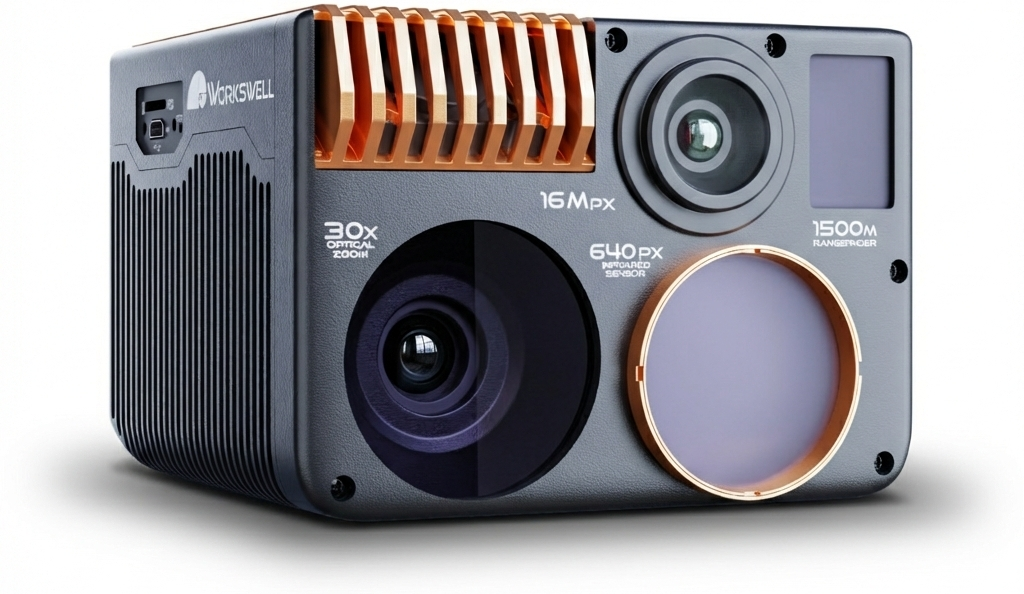
\includegraphics[width=0.45\textwidth]{images/wiris_enterprise_shadow.png}
    \vspace{-1em}
    \caption{
        The Workswell WIRIS Enterprise multi-sensor system.
        \cite{worksellWIRISspec2022}
    }
    \label{fig:WIRIS_Enterprise}
\end{figure}

\section{System Integration Overview}

% Table for weight

% Table for power consumption

% Figure for single-drone system architecture


\newpage
\chapter{Sensor Fusion}
\label{chap:sensor_fusion}

sources: 
A systematic literature review on object detection using near infrared and
thermal images (Drive) - late part of the paper, where they compare early, mid and late fusion approaches

% Use end of introduction to motivate sensor fusion \cite{bustos2023reviewObjectDetectionIR}
% Use section 6 for fusion approaches \cite{bustos2023reviewObjectDetectionIR}
% Use section 7 for challenges \cite{bustos2023reviewObjectDetectionIR}

\section{Motivation for Sensor Fusion}

Maybe put in the hardware chapter when we talk about selection
of sensor modalities, but also here in the sensor fusion 
chapter, we can talk about the motivation for sensor fusion.

\section{Problems in Sensor Fusion}

Fusion Degradation - Rethinking Multi-modal Object Detection from the Perspective of
Mono-Modality Feature Learning (Drive)

\section{Early Fusion}

\section{Mid (Feature-level) Fusion}

\section{Late Fusion}


\newpage
\chapter{Object Detection}
\label{chap:object_detection}
Lorem ipsum

\section{Single Stage Detectors}

\section{Two Stage Detectors}

\section{Tracking-by-Detection}


\newpage
\chapter{Dataset}
\label{chap:dataset}
Lorem ipsum

\newpage
\chapter{Detection Implementation}
\label{chap:implementation}

Lorem ipsum

\section{RGB-Thermal Fusion}

\section{Distance Sensor integration}

\section{Edge Optimization}


\newpage
\chapter{Evaluation}
\label{chap:evaluation}
Lorem ipsum


\newpage
\chapter{Limitations}
\label{chap:limitations}
Lipsum \ldots

\newpage
\chapter{Conclusion and Future Work}
\label{chap:conclusion}

\newpage

%
% agsm in der uibk vorlage
%
% ^.

\bibliographystyle{agsm} %apalike
\bibliography{literatur}


\end{document}
